\section{User Interface Software Suite}\label{sec:ui}

A standardized graphical user interface (GUI)\footnote{GUI is synonymous with Operator Control Unit (OCU).} was developed to be robust, intuitively usable by anyone, and serve as an all-in-one software suite (Fig. \ref{fig:gui_flow}) for servicing inputs and outputs via a middleware, called Robot Operating System (ROS), which acts as the backend of the GUI. The GUI frontend, as seen by the user, is responsible for relaying environmental sensor and navigation data. The GUI software backend is standardized for use on any ground robot that is able to traverse through a 3 degree of freedom (DOF) work space ($x$,$y$,$\theta$) using an under-actuated controller. The user is able to control the robot's movement with a single virtual joystick for controlling both forward motion and turning motion. A wrapper is written to translate the joystick commands to actual motor commands. A second virtual joystick is available and dedicated to manipulating the camera viewpoint towards regions of interest in real time. This secondary joystick allows the user to control a pan-tilt unit attached to the camera base. The shared bandwidth for camera feed and joystick commands is automatically adjusted and delegated based on the bandwidth that is available at a particular instance in the wireless connection from the robotic platform to the control unit. The GUI will alert the user if any bandwidth limits have been reached, and will attempt to provide the user with the most up-to-date sensor and video data, allowing the user to make the most informed decisions possible in a given situation. Bandwidth concerns have a real impact upon mobile safety applications and must be taken into account; \cite{erikson2013} goes into further detail about how mobile constraints can alter the user interface and backend.

\begin{figure}
	\centering
	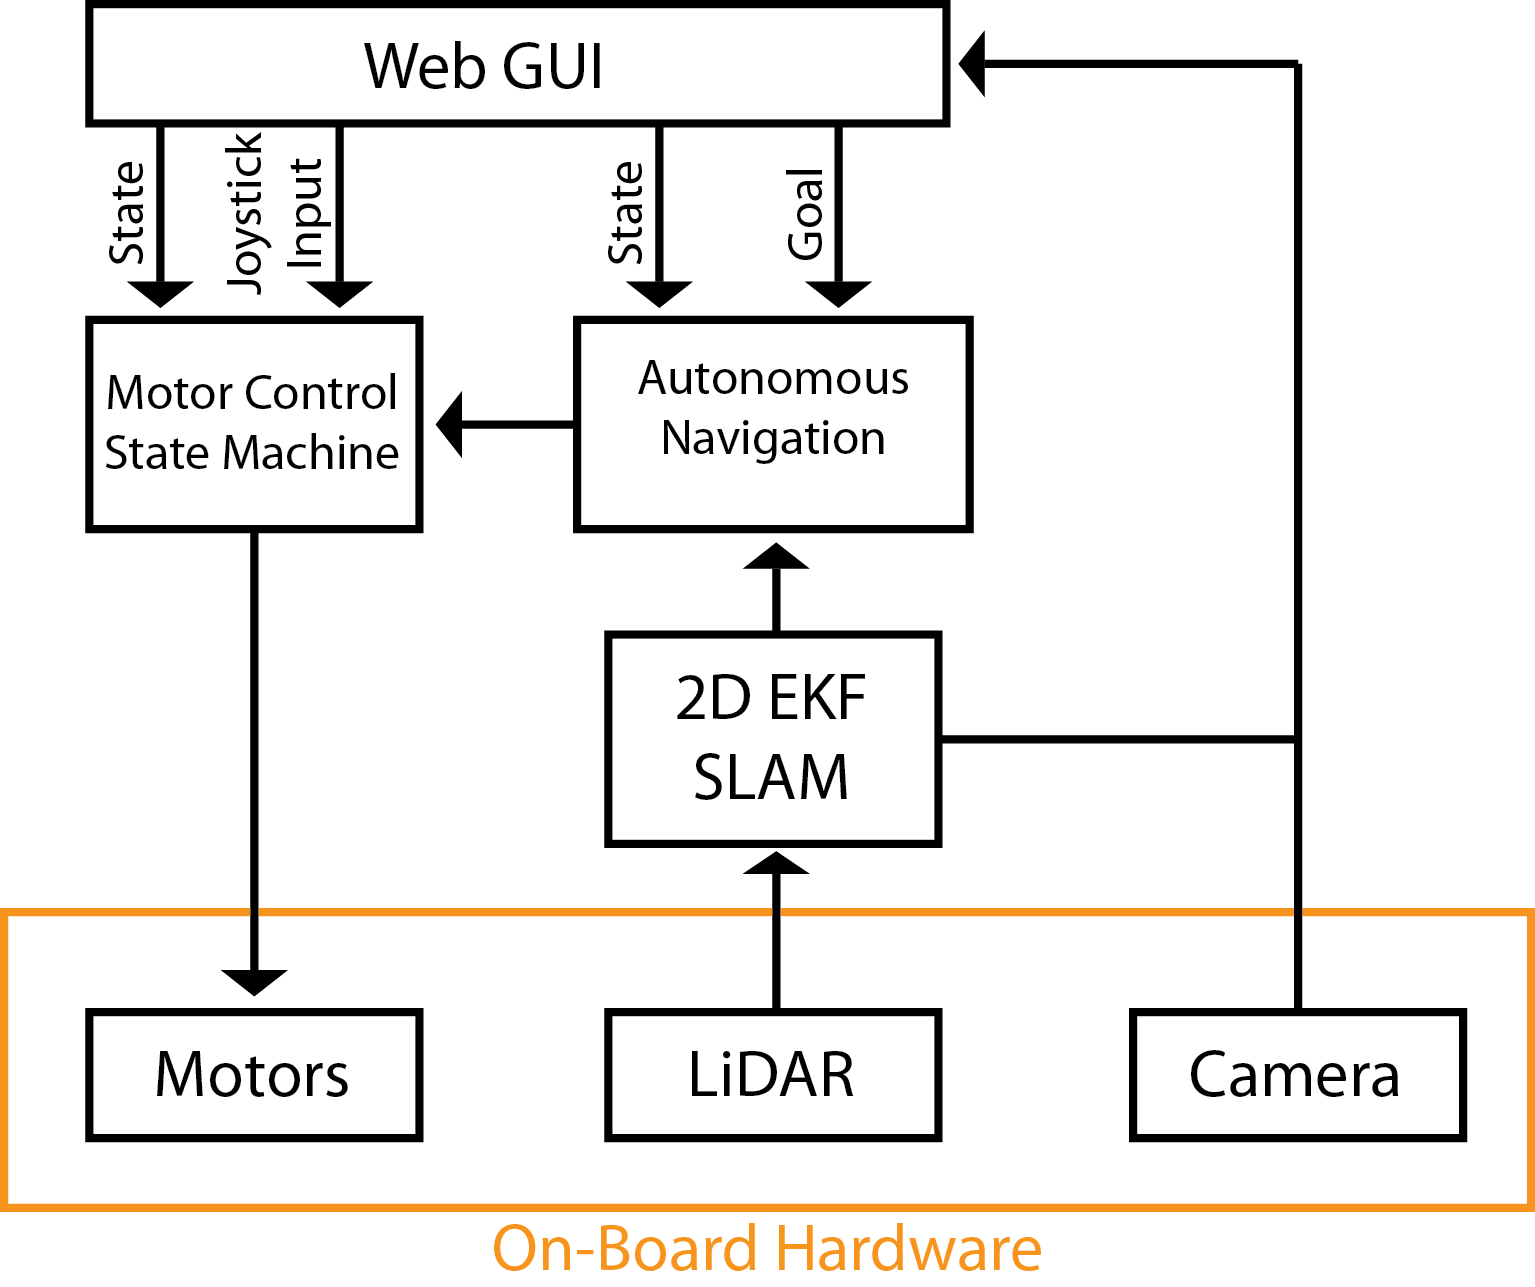
\includegraphics[width=0.48\textwidth]{pictures/Korpela_GUI.png}
	\caption{System flow of individual robot interface.}
	\label{fig:gui_flow}
\end{figure}

%To use this GUI for other ground robot platforms, all that would need to be developed is the wrapper code that translates the joystick into movement, assuming a different robot platform will have a different language coded onto its on-board system or motor controller. 

%While the control unit can be anywhere in the world, thus allowing the robot user to operate it through the internet or cloud service, there is better overall performance as well as lower latency in video stream, sensor data, and joystick data when the control unit is within the same compound as the robot. In ideal conditions, the user would be able to see and respond to any obstacle that is close by within low response time deltas, however under most conditions this isn't possible nor reasonable to expect. Low level obstacle avoidance function aids with basic navigation and reduces the probability of a crash that may be unforeseen by the user. The risk of the robot crashing into an obstacle cannot be completely mitigated because of several factors, but a few are real world delays in the data stream, loss of user's focus, lapses in data due to packet loss, the camera view is facing away from the obstacle, and connection loss.

%Another feature that has been built into the GUI is controlling based on way points instead of direct control over the robot. This allows for the user to click on the map to command the robot to navigate to the destination if possible. A 2D map is generated using SLAM from a LIDAR mounted on the robot--only differentials in the map are sent over the network. So while the initial connection may be slow, the delay during use is reasonalble. The 2D point that the user inputs is then fed into the navigation stack to attempt to reach the end goal. A third mode that the robot can be put into is pure autonomous navigation where the user can view what the robot is doing but won't have any control over the robot. The controller's multiple functionality allows for the user to pick the most appropriate mode of operation for a particular point in time, or to help the robot if it ever gets stuck. This is an important consideration when developing a GUI that is meant for long term industrial use, as all robots will eventually encounter something that they don't know how to deal with. 

\subsection{Navigation Modes}

As previously mentioned, the GUI allows the user to utilize two joysticks with one being for robot motion, and the other for camera pan-tilt motion; this two joystick scheme constitutes the first control mode. The GUI is designed to feature additional control modes. The control modes change the level of autonomy the robot exhibits during its mission. This feature, of course, requires for the different control modes to be hard-coded into the robot to ensure full functionality, both in terms of autonomous motion and safety of equipment in the facility being traversed. The change in control modes helps reduce the probability of mission failure or loss of robot if the control unit loses connection to the robot. The modes also change the level of involvement of the user in navigation duties, thus allowing the user to focus on higher level duties such as finding sources of contamination. This reduction of mental fatigue on the user helps increase mission success rate. All navigation modes utilize the GUI's built-in features of map updating when differentials are found, obstacle proximity alerts, and environmental sensor warnings. 

% or thorough sterilization of the robot's local environment
%The second navigation mode provided through the GUI lets the user move the robot via way point navigation, which is done through a 2-Dimensional (2-D) interactive map of the compound that is provided to both robot and control unit prior to start of the mission. The robot is given way point locations to reach on the interactive map by the user during the start of its mission to alleviate future bandwidth needs that may arise as the mission progresses, and as bandwidth becomes restricted with increased distance from the control unit. These way points are generated by the interactive map feature after translating user input given via a mouse click-action on the 2-D map. If, for any reason, the robot is incapable of navigating to a way point it sends a warning message to the user indicating that autonomy has been reduced, and the robot has reverted back to control mode 1. The user can then use 2 joysticks to manually  maneuver the robot further into the compound or return it to the start point. After a predetermined amount of time, with no user input in control mode 1, the robot elevates autonomy and reverses course to return to the mission's start position using the way points taken to arrive at its current position. 

The second navigation mode allows for full autonomous exploration of the environment regardless of having any \emph{apriori} knowledge of the environment or not having a map. The robot uses LIDAR-based SLAM-EKF \cite{weingarten2005ekf, castellanos2007robocentric} to generate a map if none exists already. The map data is held in the on-board PC of the robot and can be transmitted on demand or streamed live. All navigation and obstacle avoidance actions are recorded on the full 3-D map, as metadata, that is generated as the robot progresses through the environment. Video data can also be toggled on if the user desires to visually inspect mission progress. By default, in order to reduce bandwidth saturation, map data is not transmitted to let mission critical sensor data take transmission priority.  A fail-safe feature sends a warning message to the user to indicate that the robot has reverted back to Mode 1 for manual navigation. This only occurs if the robot is unable to continue through the environment or has encountered a navigational error in its on-board programming. If the user takes no action or the connection has been lost, the robot again elevates autonomy to its original setting to reverse course and return to the mission start position. 

\subsection{HTML Interface}

The desire to create a web-based control application has been explored since the inception of the Internet which is further described by use cases provided in \cite{goldberg2002beyond}. The GUI is a web application that has all the mentioned features to be toggled on or off through a settings window which is separate from the main robot interaction window in order to reduce the clutter the user sees while performing a mission (Fig. \ref{fig:gui_screenshot}). This will reduce the likelihood that the user will mistakenly click or press the wrong button during mission critical moments. The aforementioned navigation modes can be toggled on-the-fly by the user and are accessible directly from the main robot interaction window. The GUI frontend itself is based on Robot Web Tools \cite{webtools,lee2012web} which is a set of modules that help create web-based robot control applications. It allows ROS software package messages and topics to be accessible through a web interface that is constructed using HTML5 and Javascript via a wrapper called \textit{rosjs} \cite{osentoski2011robots}. The GUI is essentially a web accessible overlay that allows the user to send and receive data across a connection between a ROS server, the control unit, and its corresponding ROS client, the robot. The advantage of using HTML5 is its cross-platform compatibility allowing the web application to be used by PCs, tablets, and smart phones \cite{hilton2014lightweight}. On the ROS client, the robot computer runs a \textit{roscore} node that utilizes a package called \textit{rosbridge} which allows socket-based access to ROS through Javascript \cite{crick2011rosbridge}.

\begin{figure}
	\centering
	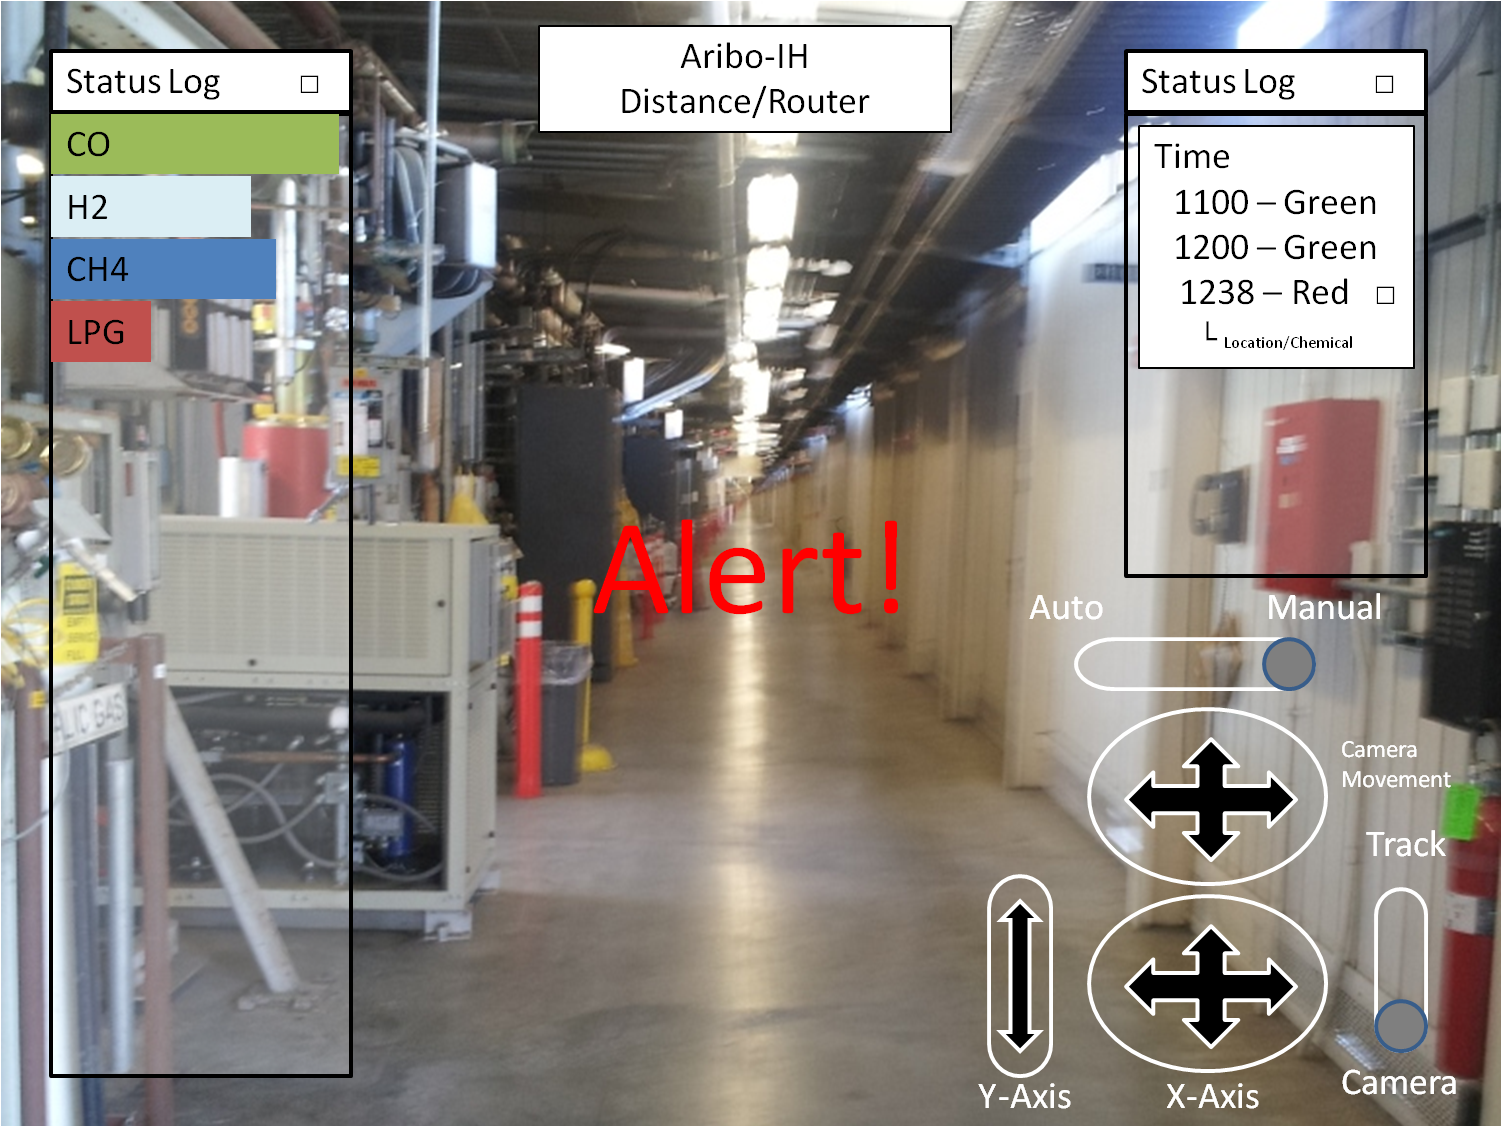
\includegraphics[width=0.48\textwidth]{pictures/gui-slac.png}
	\caption{Screenshot of the developed web-based GUI allowing for view of the camera and 2-D map.}
	\label{fig:gui_screenshot}
\end{figure}
